\chapter{Network Compression}
The size of deep neural networks has been a major hindrance to their implementation on resource constrained hardware devices. The weight matrix sizes consume significant storage and memory bandwidth. Changes on an algorithmic level have been proposed extensively in the last couple of years with regards to reducing the model sizes of deep neural networks. Reducing the number of parameters, not only allows for faster and less distributed training, but for more power-aware inference which is the aim of our work.\\
Compression of a network, as discussed above, is the reduction of the number of parameters in the model/network. The method of reduction of parameters influences the training method in a unique way ie, the training phase is aware of the compression and must account for the model changes. From recent literature, two broad paradigms have emerged, namely:
\begin{enumerate}
    \item Low Displacement Rank Networks
    \item Pruning and Quantization
    \item Knowledge Diffusion
\end{enumerate}

\section{Low Displacement Rank Networks}

This method of compression takes advantage of the structured nature of certain types of matrices to reduce the number of unique parameters from On2 to On. This not only reduces the storage complexity from On2 to On, it also reduces, due to fast matrix multiplication methods, the computational complexity roughly from On2 to Onlogn or Onlogn2. It uses the fact that any matrix can be compressed to a Low Displacement Rank matrix M which after being computed using the appropriate operation, is decompressed back to the desired result. For deep neural networks, an error bound has been proven for such approximations on the performance of a neural network. \\
Examples of structured matrices are: Circulant, Toeplitz, Henkel, Vandermonde, Cauchy. The predictable structure of these matrices reduces the number of parameters and also eases the indexing process due to its predictability, a lack of which affects the first two methods hence increasing the potential optimization that is possible beforehand when designing an ASIC/FPGA implementation. The other added advantage with respect to the pruning method elaborated below is that there is no iterative training process after introducing the compression as the entire training mechanism is aware of the exact structure of the matrix from the beginning. A recent work uses Circulant matrices as suggested to train the network and achieve a significant speedup on their FPGA implementation of LSTMs.


\section{Pruning and Quantization}
\subsection{Pruning}
In a trained neural network, the weight matrix consists of parameter values that vary drastically in magnitude. Similar to the connections amongst neurons, according to the function that the network is trying to imitate, only certain connections are of computational importance. Hence those connections that have a small magnitude can be removed to increase the sparsity of the network. The state-of-art implementation of such a deep neural network pruning scheme is Deep Compression. We will illustrate the technique suggested and adopt the same to reduce the network size and also explore the different avenues of optimization this creates in the Distributed Arithmetic section.\\
Procedure in training phase: (flow chart insert if possible):
\begin{enumerate}
    \item Train the network at its full capacity.
    \item Prune small magnitude connections by setting a threshold.
    \item Retrain the remaining connections for fine-tuning.
\end{enumerate}

\begin{figure}[h] 
	\caption{A $4X4$ matrix pruned with a threshold magnitude of 0.25}    
    \centering
    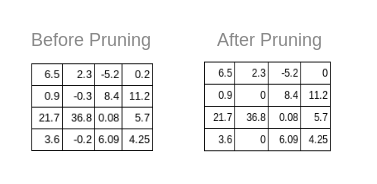
\includegraphics[width=0.25\textwidth]{pruning}
\end{wrapfigure}

\subsection{Quantization}
Further reduction of the model size is possible by quantizing the remaining parameters to K levels. The standard procedure to do this is through K-means clustering. Therefore only logK bits will be required to store the parameters. Literature shows that the two practices of pruning and quantization can be combined together to provide significant drop in the model size. Although the practice of quantization is helpful in reducing the storage bandwidth, it is yet to be used as an way to reduce the implementation of the network. 



